\documentclass[
polish,
xcolor={svgnames,pdftex,table},
mathserif,
11pt,
hyperref={pdfpagelabels=false},
%handout,
presentation,
]{beamer}
% ponizej opcja, zeby pdflatex honorowal grafike w PDFach w wersji 1.5
%\pdfminorversion=6 




\usepackage[polish,english]{babel}
\usepackage{xmpmulti}
\usepackage{amsmath}
%\usepackage[MeX]{polski}
\usepackage[T1]{fontenc}
\usepackage[cp1250]{inputenc}
\usepackage[OT4]{polski}
\usepackage{graphics}
\usepackage{relsize}
\usepackage{listings}

\usepackage{booktabs}
\usepackage{multirow}
\usepackage{array}
\usepackage{color}
\usepackage{alltt}
\usepackage{verbatim}
\usepackage{wasysym}

\usepackage{pgfpages}
\hypersetup{pdfpagemode=FullScreen}

\mode<presentation>
%{
%\definecolor{frameheadforeground}{RGB}{169,33,62}
%\definecolor{frameheadbackground}{RGB}{255,255,255}
%\setbeamercolor{structure}{fg=frameheadforeground,bg=frameheadbackground}
%\setbeamercolor{headline}{parent=palette quaternary}
%\setbeamercolor{footline}{parent=palette primary}
%\setbeamercolor*{palette quaternary}{fg=black,bg=white}
%\usetheme{Boadilla}
\usetheme{Singapore}
%usetheme{Hannover}
%\usefonttheme[mathonly]{serif}
%\usepackage{times}
%}

%\logo{
\includegraphics[height=0.5cm]{img/wne_ang.pdf}} %change here. I used an eps file logo, you can use jpg or other format

\mode<handout>
{
 \usetheme{Boadilla}
 \pgfpagesuselayout{4 on 1}[a4paper,landscape,border, shrink=2.5mm]
}



\setbeamertemplate{caption}[numbered] 

\setbeamertemplate{footline}[frame number] 
\setbeamertemplate{navigation symbols}{} %no nav symbols


%definicja zrodla
\newcommand{\source}[1]{\begin{flushleft}
\textsf{{\tiny �r�d�o: #1}}
\end{flushleft}
} 


\newcommand{\toR}{
%\subsection{Przyk�ady i �wiczenia w R}
\begin{frame}{Przyk�ady i �wiczenia w R}
\begin{center}
\includegraphics[width=0.5\textwidth]{img/toR.png}
\end{center}
\end{frame}
}

\newcommand{\putat}[3]{\begin{picture}(0,0)(0,0)\put(#1,#2){#3}\end{picture}}


\newcommand{\var}{\textrm{Var}}
\newcommand{\cov}{\textrm{Cov}}
\newcommand{\corr}{\textrm{Corr}}
\newcommand{\str}[1]{\textbf{#1}}
\usepackage{color}
\newcommand{\hl}[1]{\colorbox{yellow}{#1}}

%example
\newcommand{\EXample}[1]{\colorbox{PaleGreen}
{Example #1}
}
%exercise
\newcommand{\EXercise}[1]{\colorbox{yellow}
{Exercise #1}
}




% 20110304 wstawilem to rozwiazanie, bo wywalal mi nastepujacy blad
%Undefined control sequence:
%\beamer@frameslide ...duration=}\thispdfpagelabel
%{\insertframenumber}\xda.....
\providecommand\thispdfpagelabel[1]{}





%\title[VTS]{Range Volatility Models\\ and Their Applications in Finance}
\title[Estymatory zmienno�ci]{Efektywno�� estymator�w zmienno�ci \\opartych na zakresie zmian}
%\subtitle{}

\author[]{Pawe� Sakowski \\ \quad \\ \tiny Korefereat do wyst�pienia T. Skoczylasa ,,Modelowanie wariancji finansowych szereg�w czasowych przy u�yciu Range-based ARCH uwzgl�dniaj�cego heterogeniczno�� wariancji''}

\institute[WNE UW]{
 % Wydzia� Nauk Ekonomicznych\\
 % Uniwersytetu Warszawskiego\
}  
\date{}
\titlegraphic{
\includegraphics[width=8cm]{img/wne.pdf}}  
\date{\footnotesize Konferencja WNE UW \\Kazimierz nad Wis��\\ 27-28/9/2013}


%%%%%%%%%%%%%%%%%%%%%%%%%%%%%%%%%%%%%%%%%%%%%%%%%%%%%%%%%%%%%%%
\begin{document}
\selectlanguage{polish}
\lstset{
	language=R,
	keywordstyle=\bfseries\ttfamily\color[rgb]{0,0,1},
	identifierstyle=\ttfamily,
	commentstyle=\color[rgb]{0.133,0.545,0.133},
	stringstyle=\ttfamily\color[rgb]{0.627,0.126,0.941},
	showstringspaces=false,
	basicstyle=\small,
	numberstyle=\footnotesize,
	numbers=none, %=left
	stepnumber=1,
	numbersep=10pt,
	tabsize=2,
	breaklines=true,
	prebreak = \raisebox{0ex}[0ex][0ex]{\ensuremath{\hookleftarrow}},
	breakatwhitespace=false,
	aboveskip={1.5\baselineskip},
  columns=fixed,
  upquote=true,
  extendedchars=true,
% frame=single,
% backgroundcolor=\color{lbcolor},
}


\begin{frame}
\titlepage
\end{frame}

%\begin{frame}%[allowframebreaks]
%{Plan prezentacji}
%  \tableofcontents
%\end{frame}

%%%%%%%%%%%%%%%%%%%%%%%%%%%%%%%%%%%%%%%%%%%%%%%%%%%%%%%%%%%%%%%%%%%%%%%
\begin{frame}
\frametitle{Plan prezentacji}

\begin{enumerate}
\item Efektywno�� estymator�w zmienno�ci
\begin{itemize}
\item klasyczny estymator zmienno�ci
\item estymator Parkinsona (1980)
\item estymator Osbanda (2007)
\item estymator Garmana-Klassa (1980)
\item estymator Rogersa-Satchella (1991)
\end{itemize}
\item Uwagi do referatu Tomka Skoczylasa
\end{enumerate}
\end{frame}



\begin{frame}
\frametitle{Za�o�enia og�lne}
\begin{itemize}
\item logarytm ceny akcji podlega jednowymiarowemu ci�g�emu b��dzeniu losowemu ze sta�� dyfuzji $D$ \pause
\item a zatem, prawdopodobie�stwo tego, �e logarytm ceny $x$ znajdzie si� w przedziale $(x, x + dx)$ w momencie $t$, zak�adaj�c jego pocz�tkow� warto�� $x_0$ w momencie $t = 0$, wynosi:
$$
\Big(dx/\sqrt{2\pi Dt}\Big)\exp[-(x-x_0)^2/2Dt]
$$ \pause
\item por�wnuj�c to z rozk�adem normalnym, zauwa�amy, �e $D$ jest wariancj� zmiany logarytmu ceny $(x - x_0)$ w interwale jednostowym
\end{itemize}
\end{frame}


\begin{frame}
\frametitle{Klasyczny estymator zmienno�ci}
Tradycyjny spos�b estymacji wariancji $D$: \pause
\begin{itemize}
\item obserwujemy $x(t)$ w momentach $t = 0, 1, 2, 3, \dots, n$ \pause
\item definiujemy $d_t$ jako zmiany w $t$-tym interwale: $d_t = x(t) - x(t-1)$, $t = 1, 2, 3, \dots, n$ \pause
\item obliczamy wyra�enie:
$$
D_x = \frac{1}{n-1} \sum_{t=1}^{n}(d_t - \bar{d})^2
$$
gdzie
$$
\bar{d} = \frac{1}{n} \sum_{m=1}^{n}d_m 
$$ \pause
\item dla niskiej liczby obserwacji estymator ten ma ma�� precyzj�! \pause
%\item w wielu przypadkach $n=1$ 
\begin{itemize}
\item zmienno�� zrealizowana (Andersen \emph{et al.} 2001), 
\item modele z rodziny GARCH (Engle 1982, Bollerslev 1986 i nast�pni)
\end{itemize}
\end{itemize}
\end{frame}





\begin{frame}
\frametitle{Symulacja Monte Carlo}
\begin{itemize}
\item �cie�ka cen $x(t)$ sk�ada si� z $n = 10 000$ interwa��w, $t = 1, 2, \dots, 10000$
\item ci�g�e stopy zwrotu maj� rozk�ad normalny:
$$
\log \big [x(t)\big] - \log \big [x(t-1) \big] \sim N(0, 0.001^2)
$$
\item liczba powt�rze� symulacji = 10000 
\end{itemize}
\end{frame}



\begin{frame}
\frametitle{B��dzenie losowe}
\begin{center}
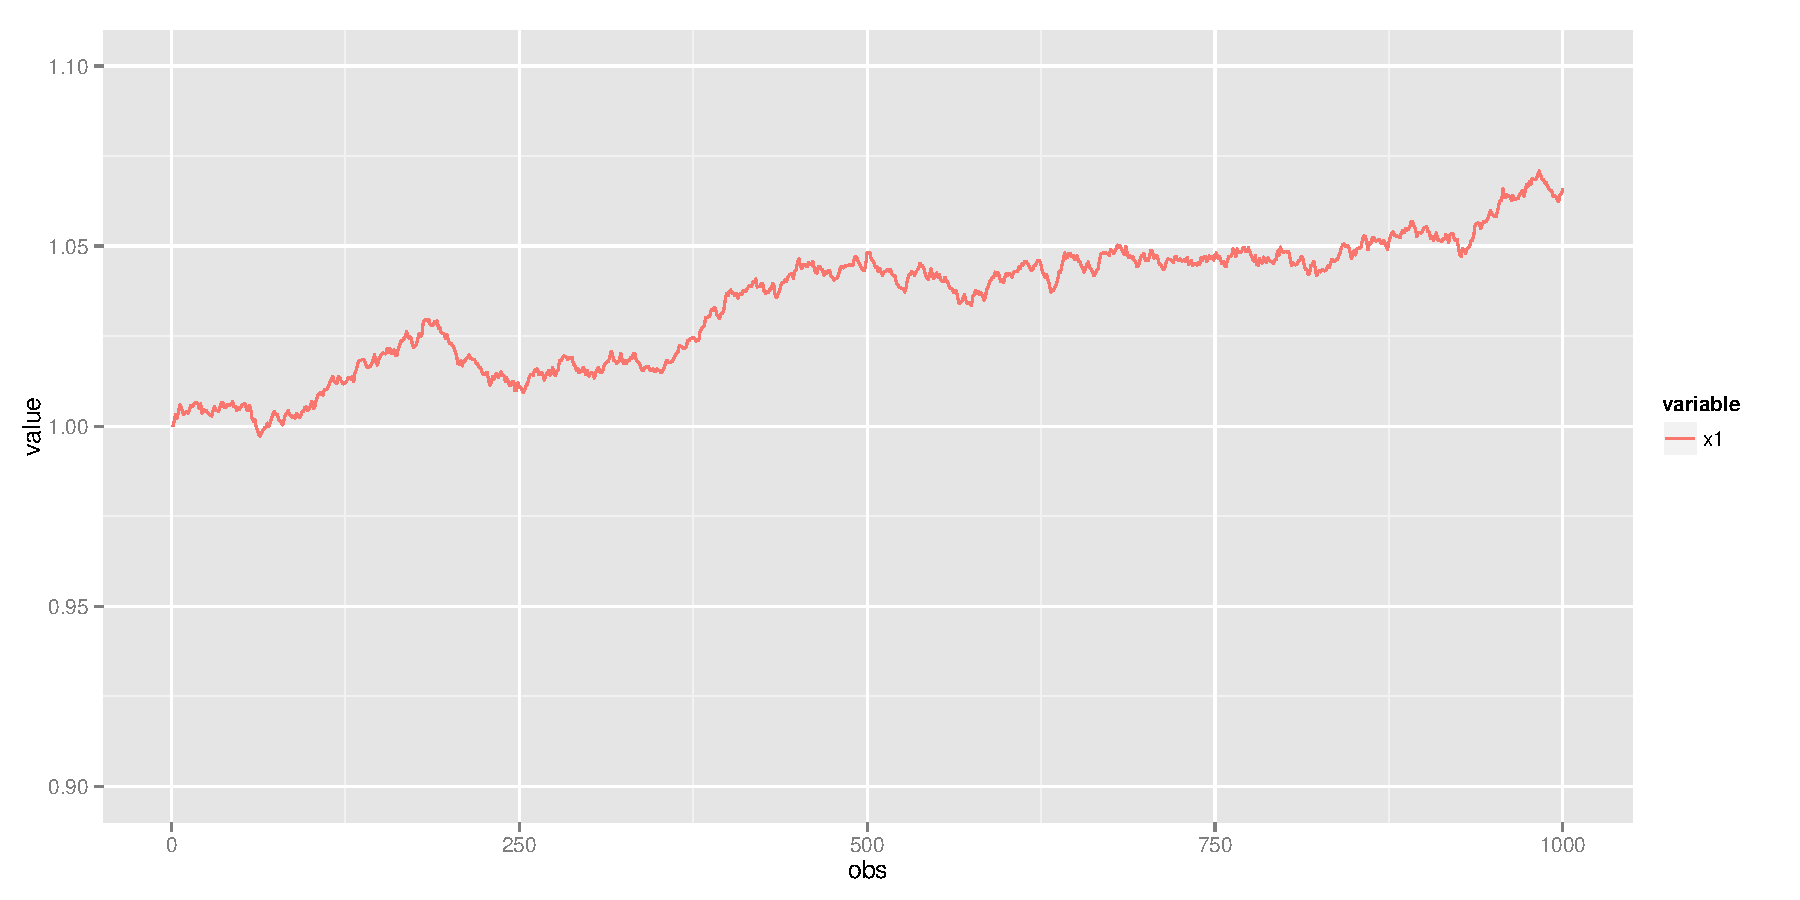
\includegraphics[width = 1.1 \textwidth]{img/rw1}
\end{center}
\end{frame}
\begin{frame}
\frametitle{B��dzenie losowe}
\begin{center}
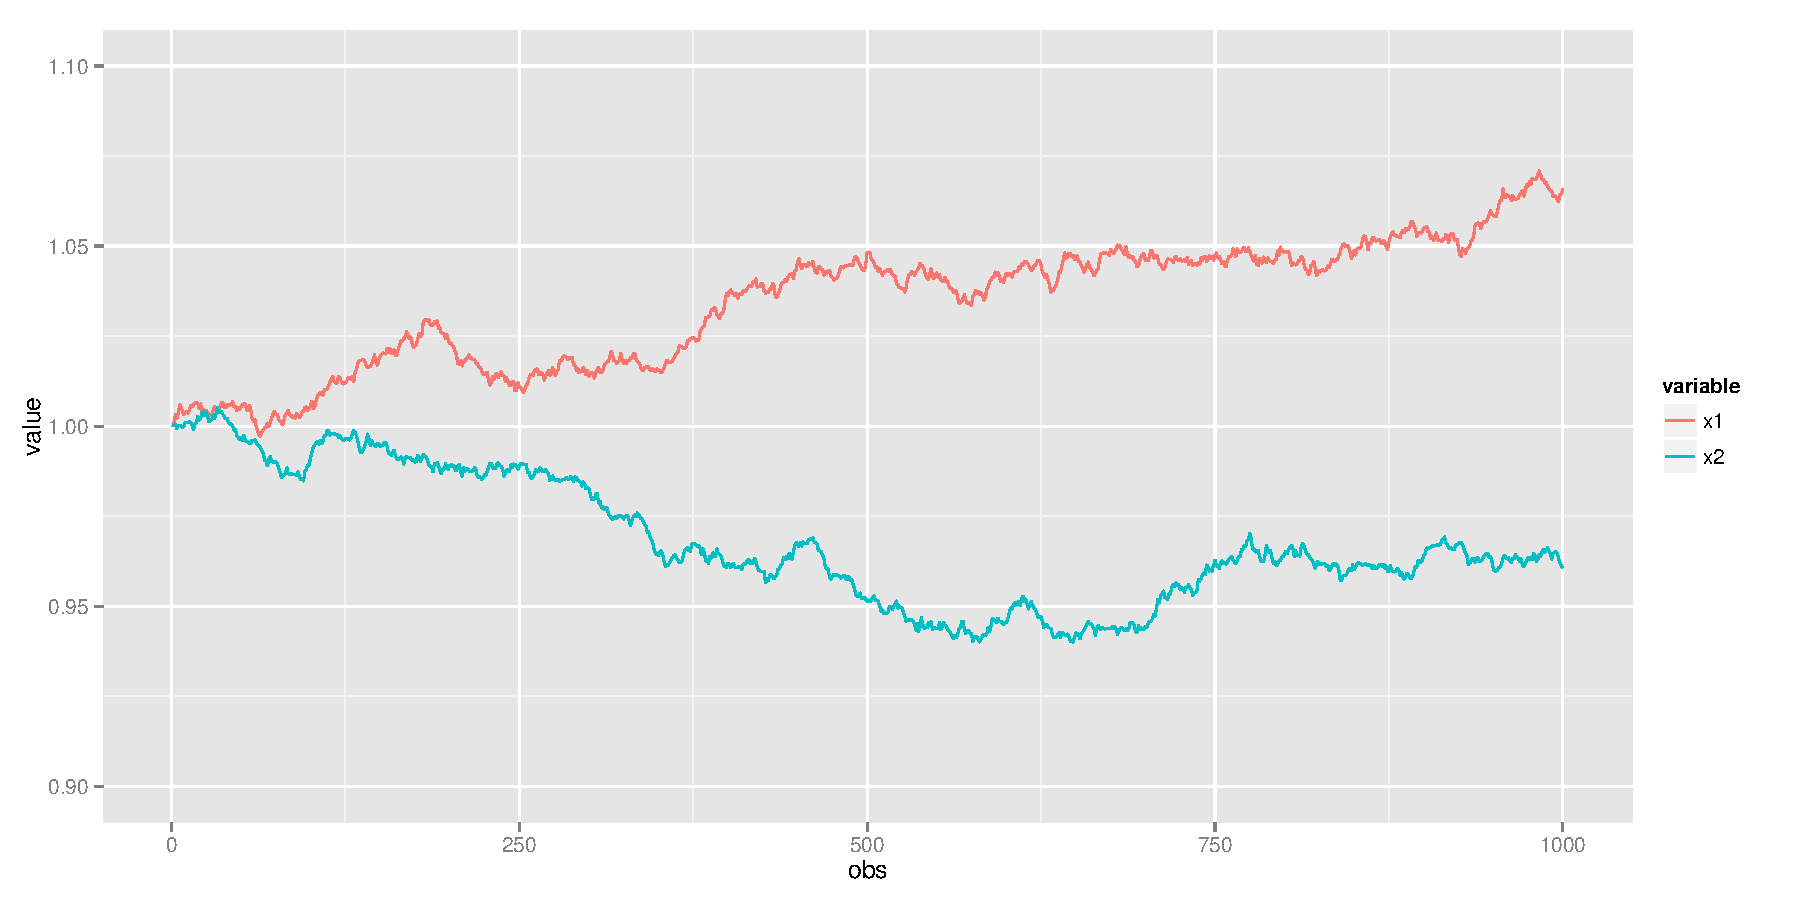
\includegraphics[width = 1.1 \textwidth]{img/rw2}
\end{center}
\end{frame}
\begin{frame}
\frametitle{B��dzenie losowe}
\begin{center}
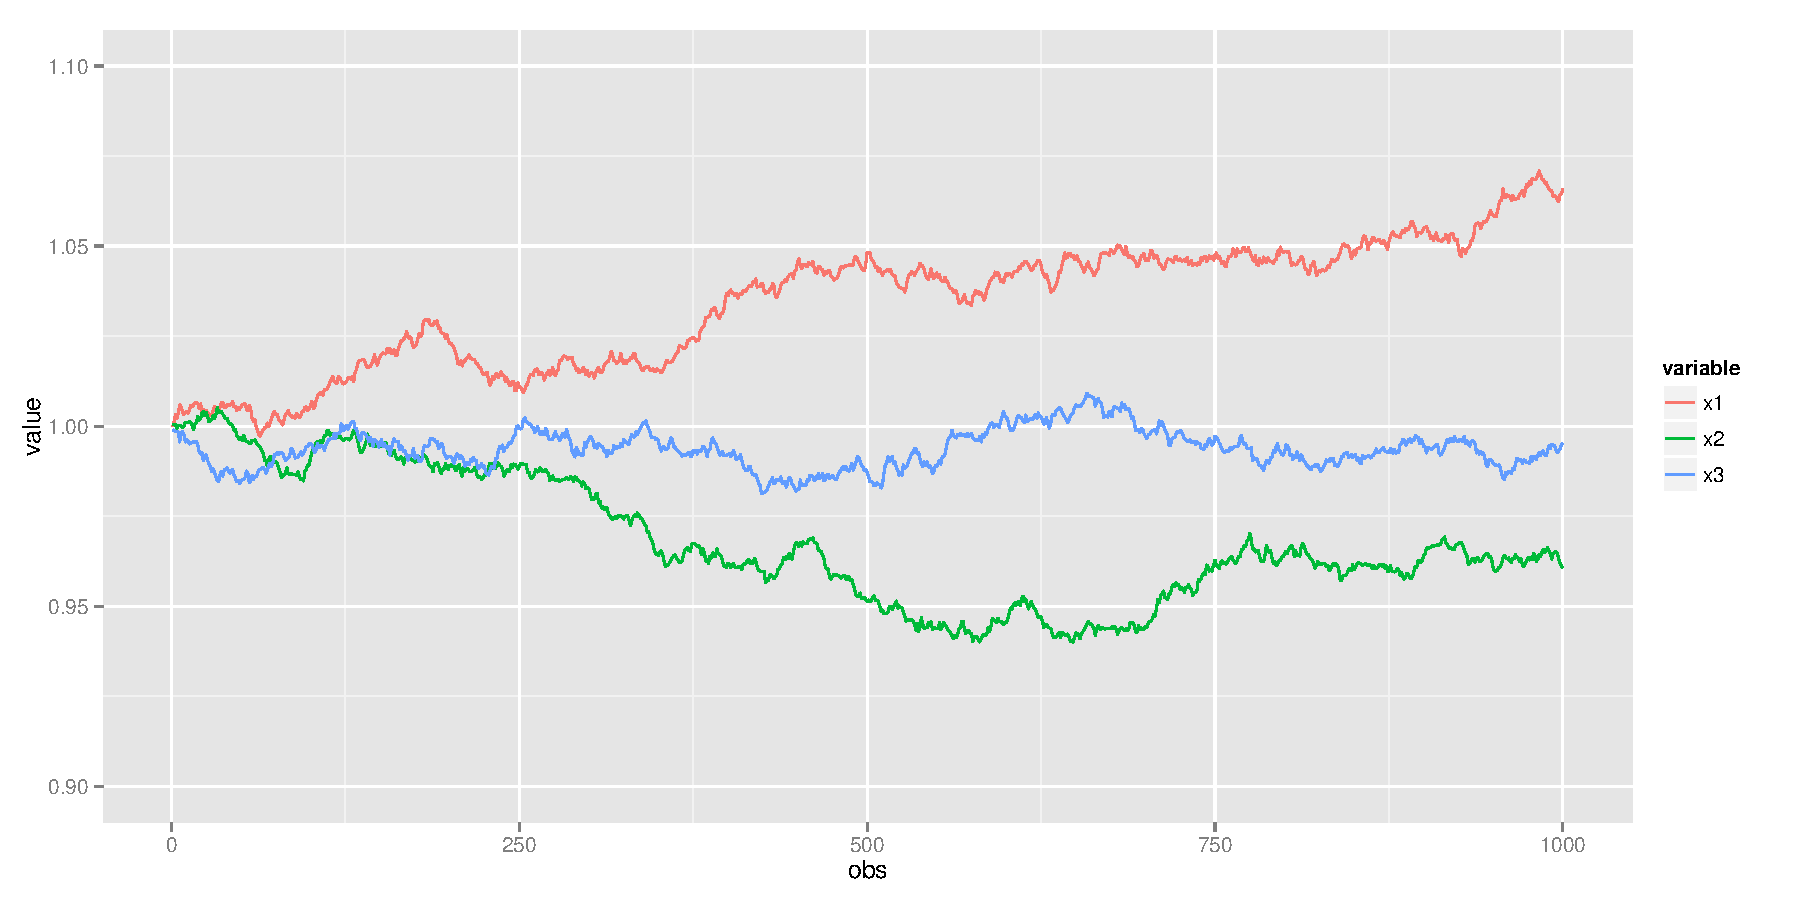
\includegraphics[width = 1.1 \textwidth]{img/rw3}
\end{center}
\end{frame}
\begin{frame}
\frametitle{B��dzenie losowe}
\begin{center}
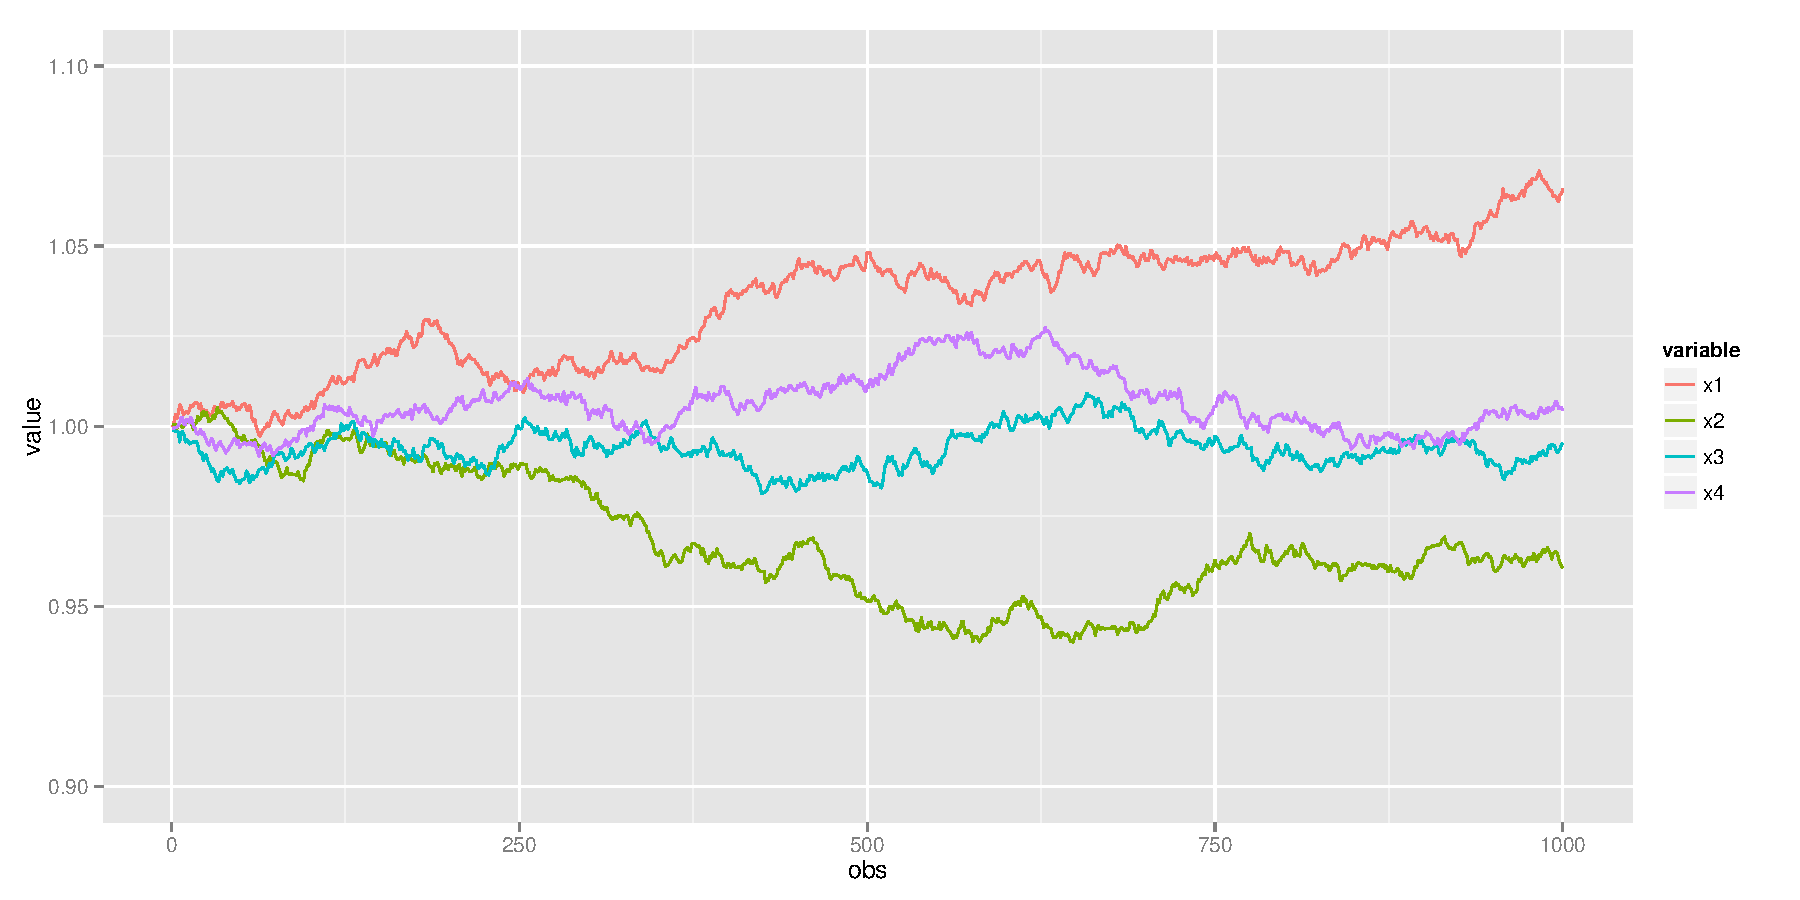
\includegraphics[width = 1.1 \textwidth]{img/rw4}
\end{center}
\end{frame}
\begin{frame}
\frametitle{B��dzenie losowe}
\begin{center}
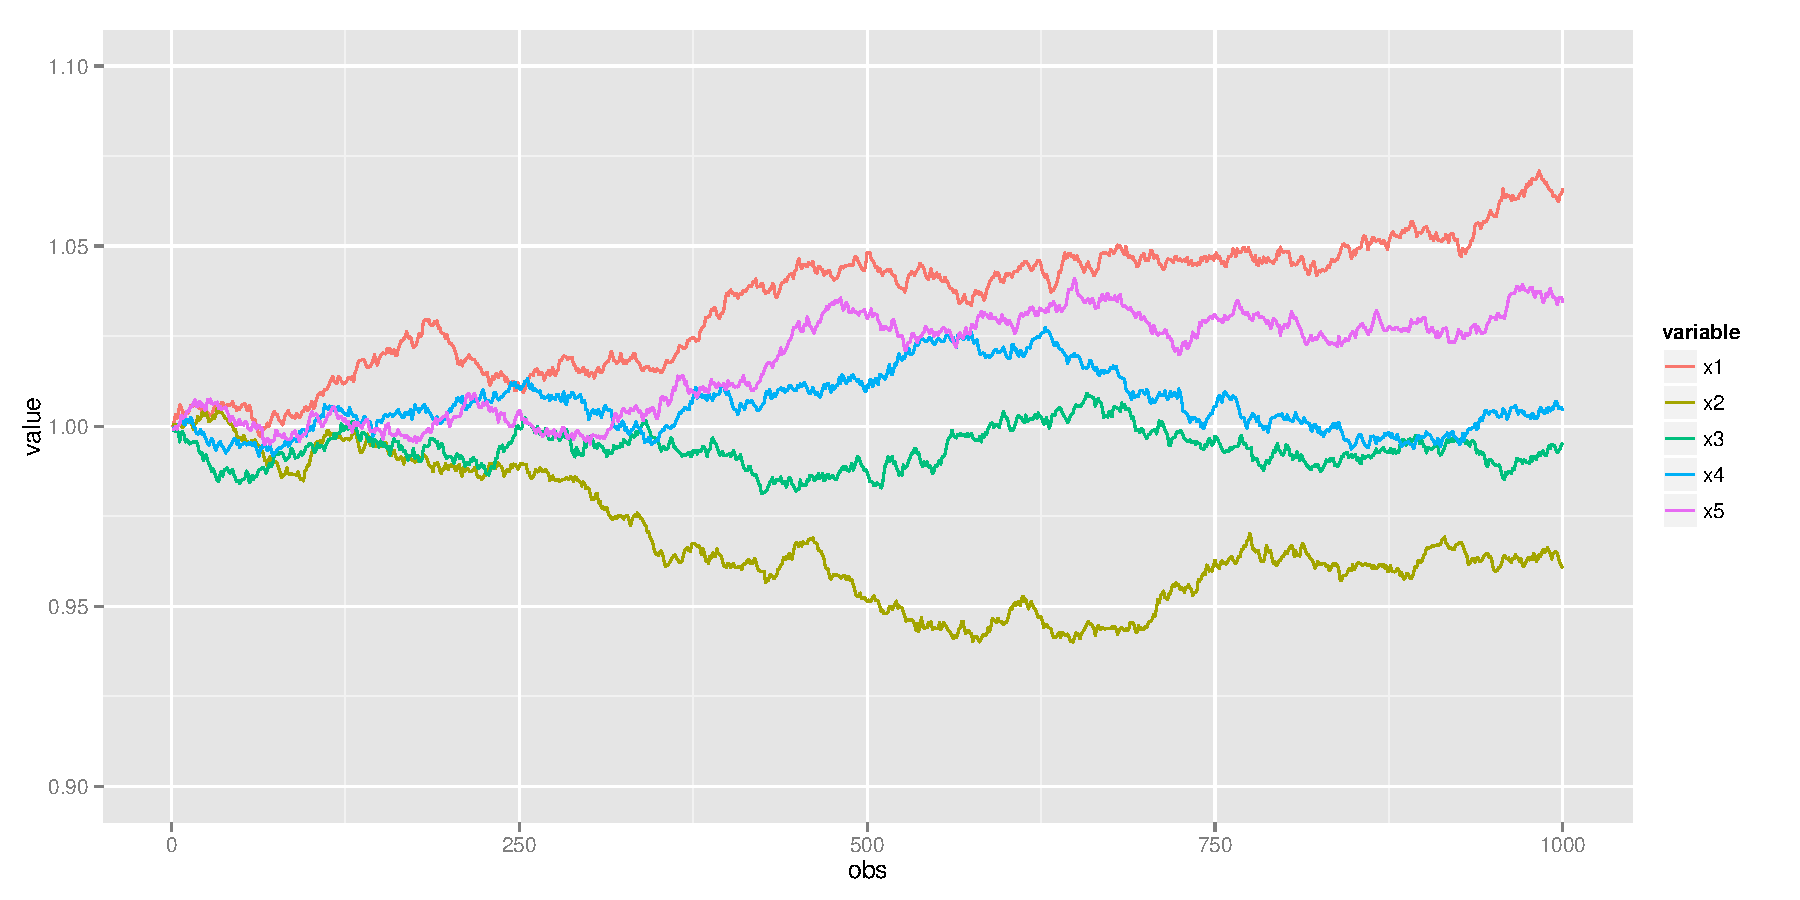
\includegraphics[width = 1.1 \textwidth]{img/rw5}
\end{center}
\end{frame}
\begin{frame}
\frametitle{B��dzenie losowe}
\begin{center}
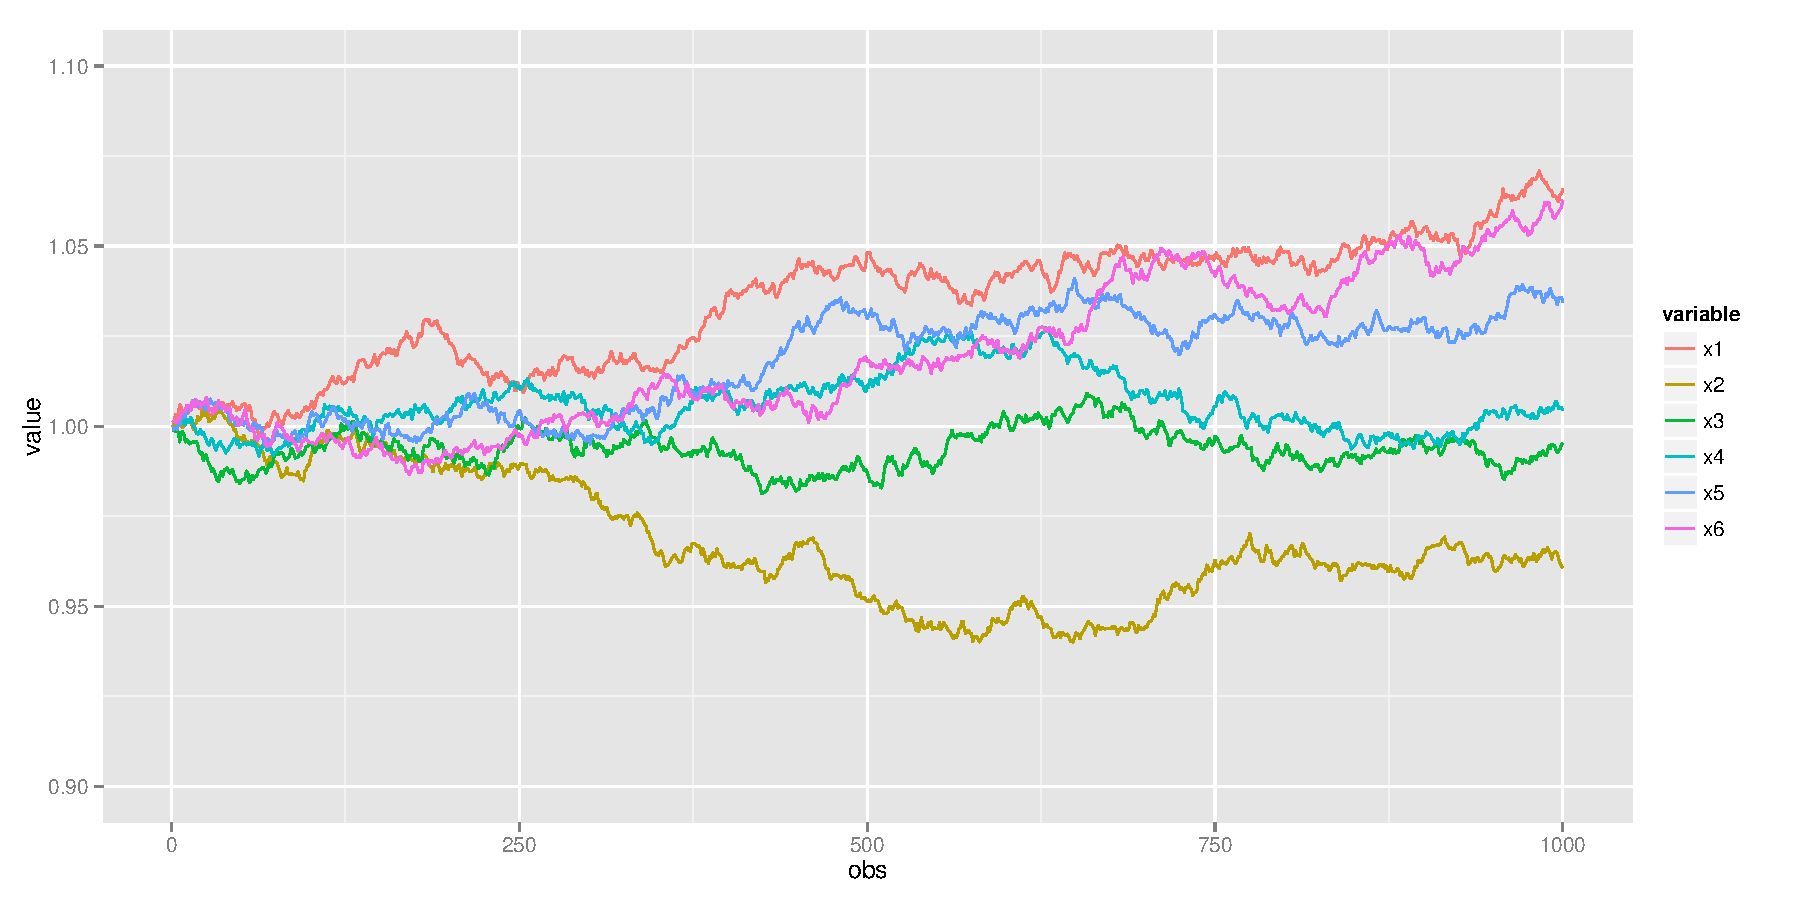
\includegraphics[width = 1.1 \textwidth]{img/rw6}
\end{center}
\end{frame}
\begin{frame}
\frametitle{B��dzenie losowe}
\begin{center}
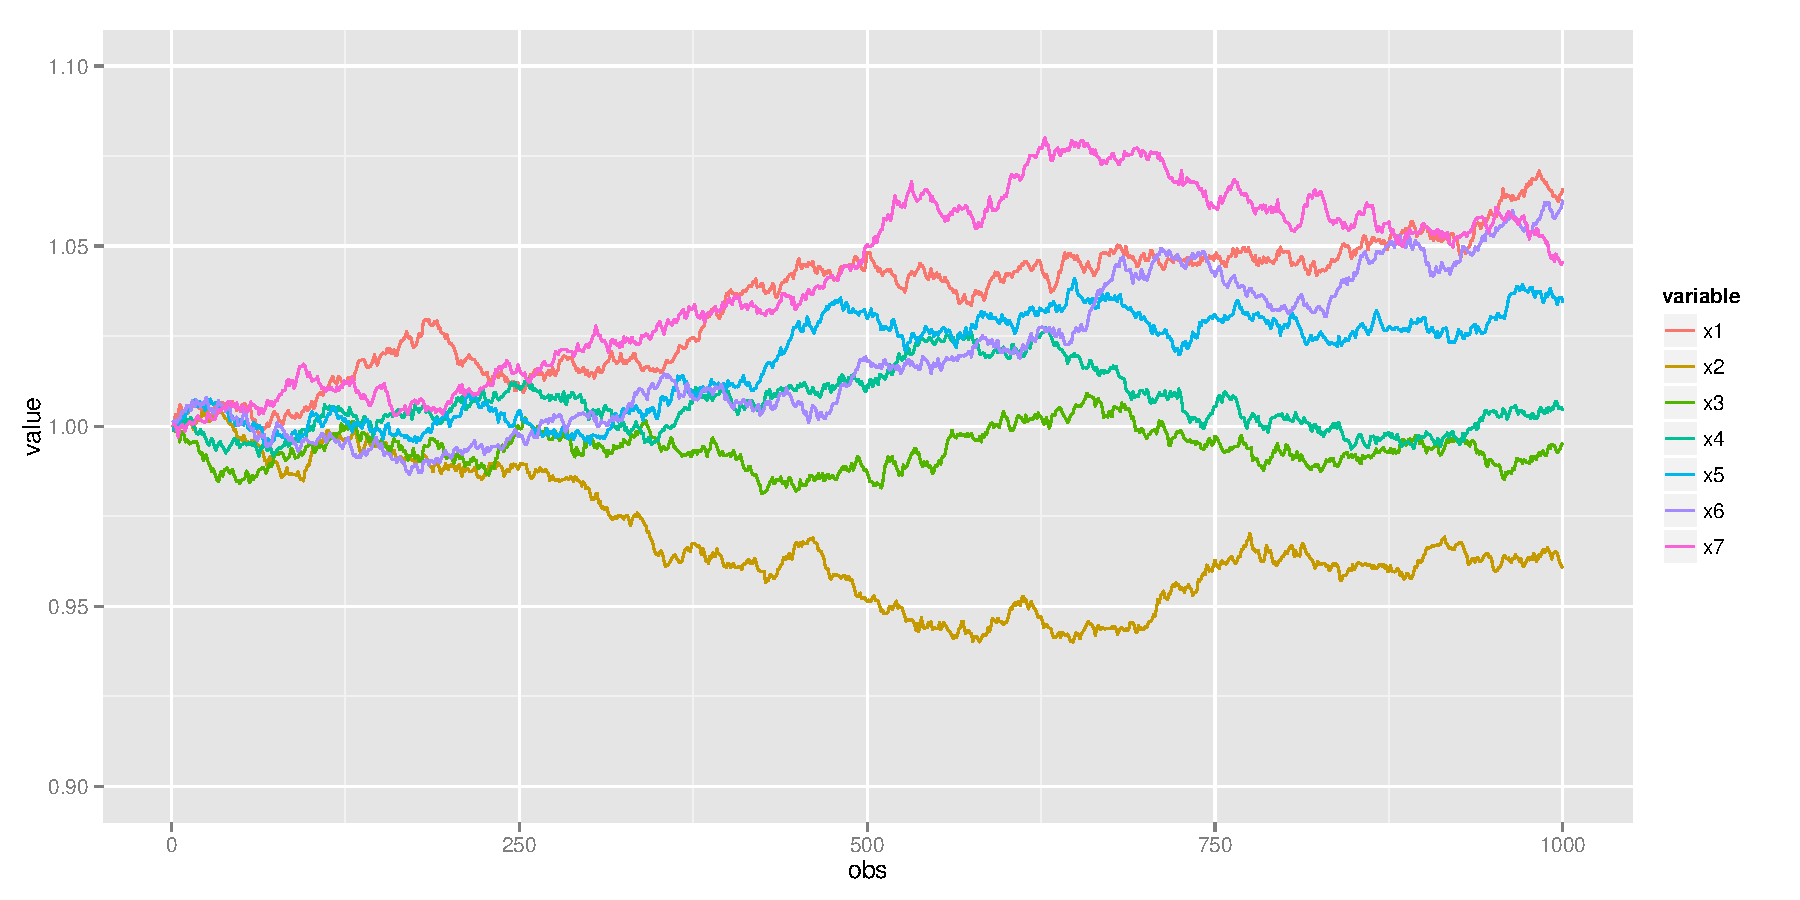
\includegraphics[width = 1.1 \textwidth]{img/rw7}
\end{center}
\end{frame}
\begin{frame}
\frametitle{B��dzenie losowe}
\begin{center}
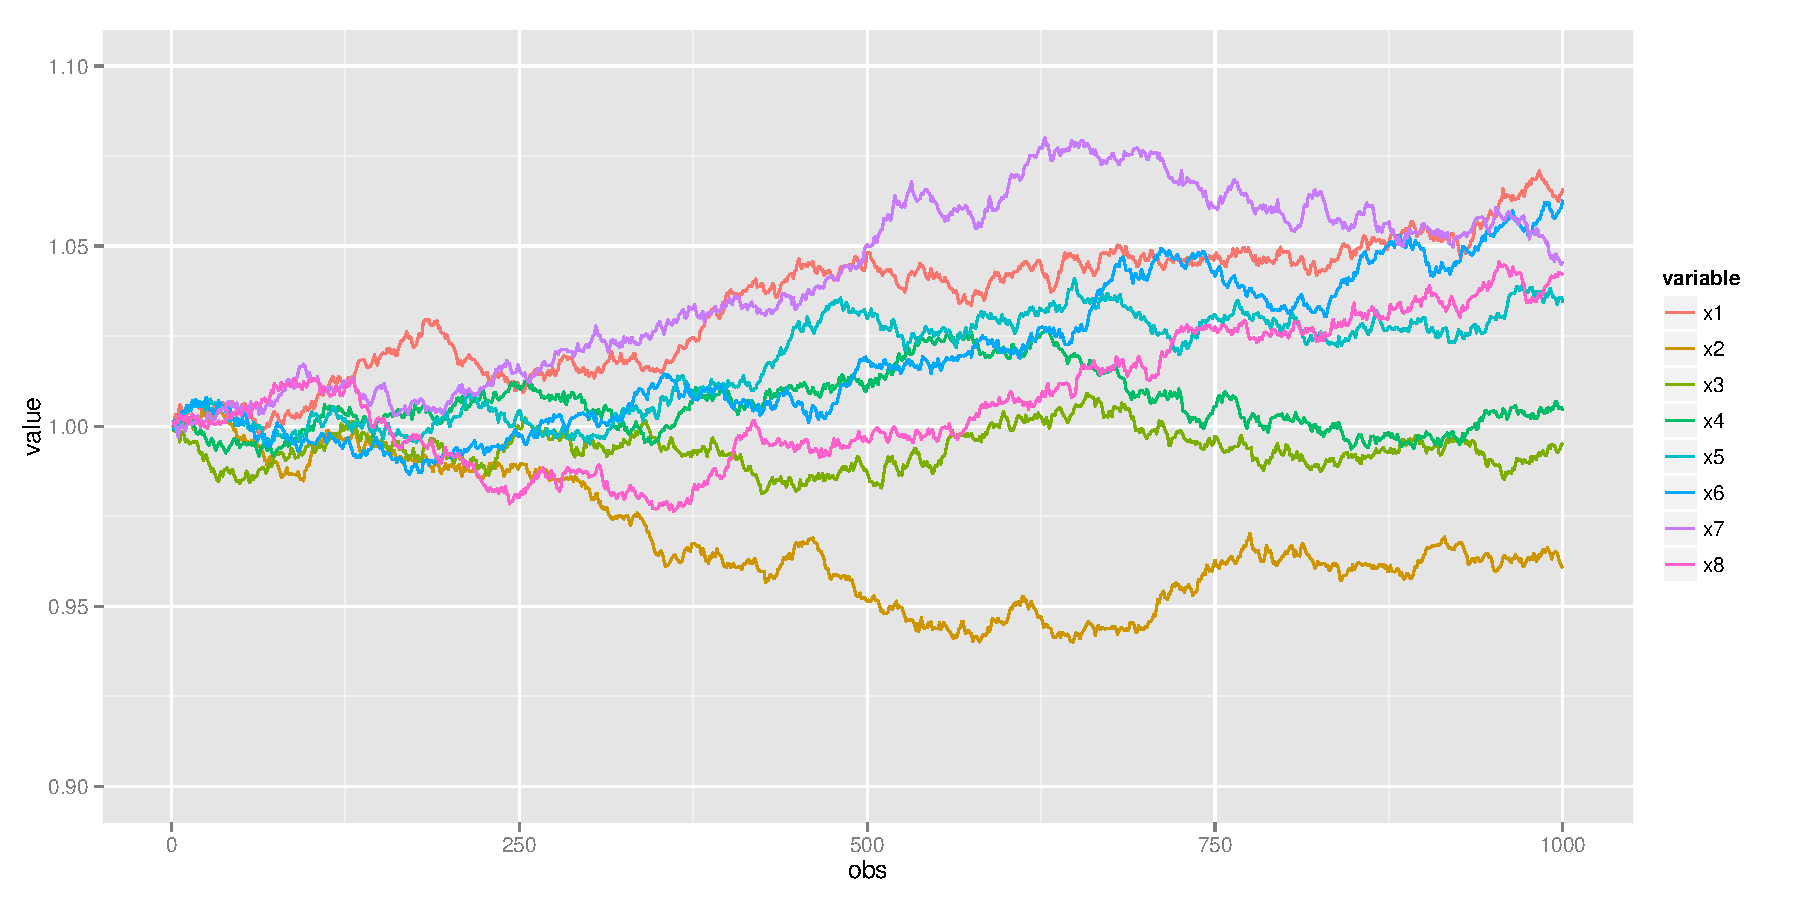
\includegraphics[width = 1.1 \textwidth]{img/rw8}
\end{center}
\end{frame}
\begin{frame}
\frametitle{B��dzenie losowe}
\begin{center}
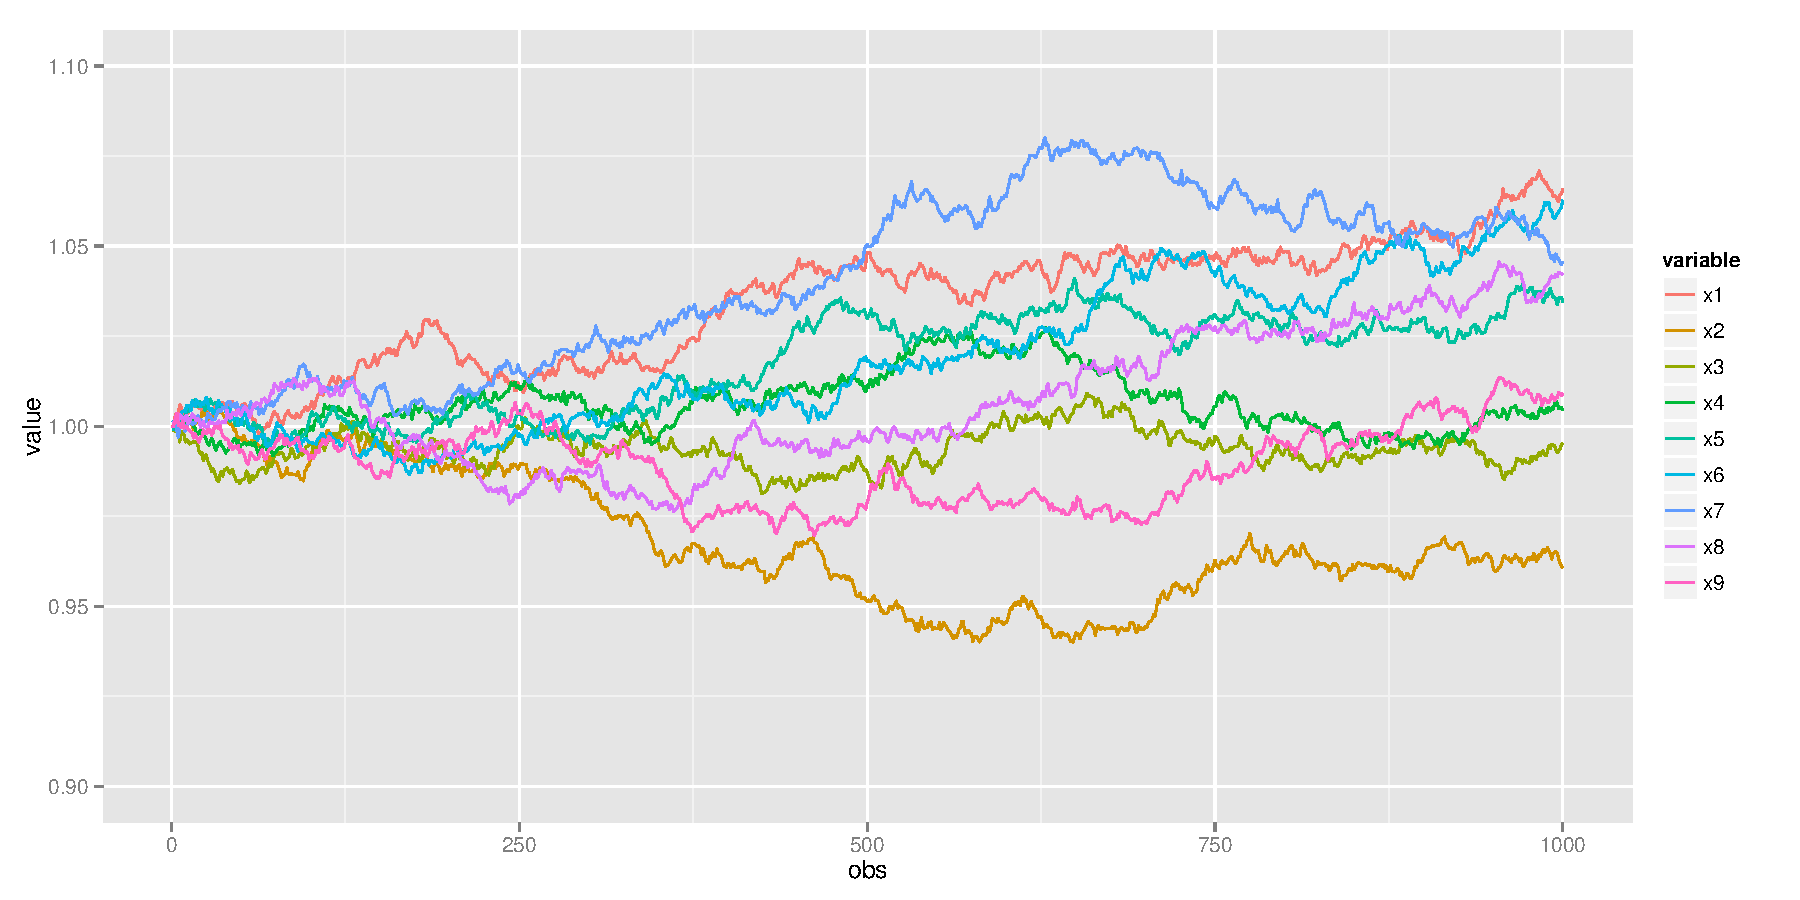
\includegraphics[width = 1.1 \textwidth]{img/rw9}
\end{center}
\end{frame}
\begin{frame}
\frametitle{B��dzenie losowe}
\begin{center}
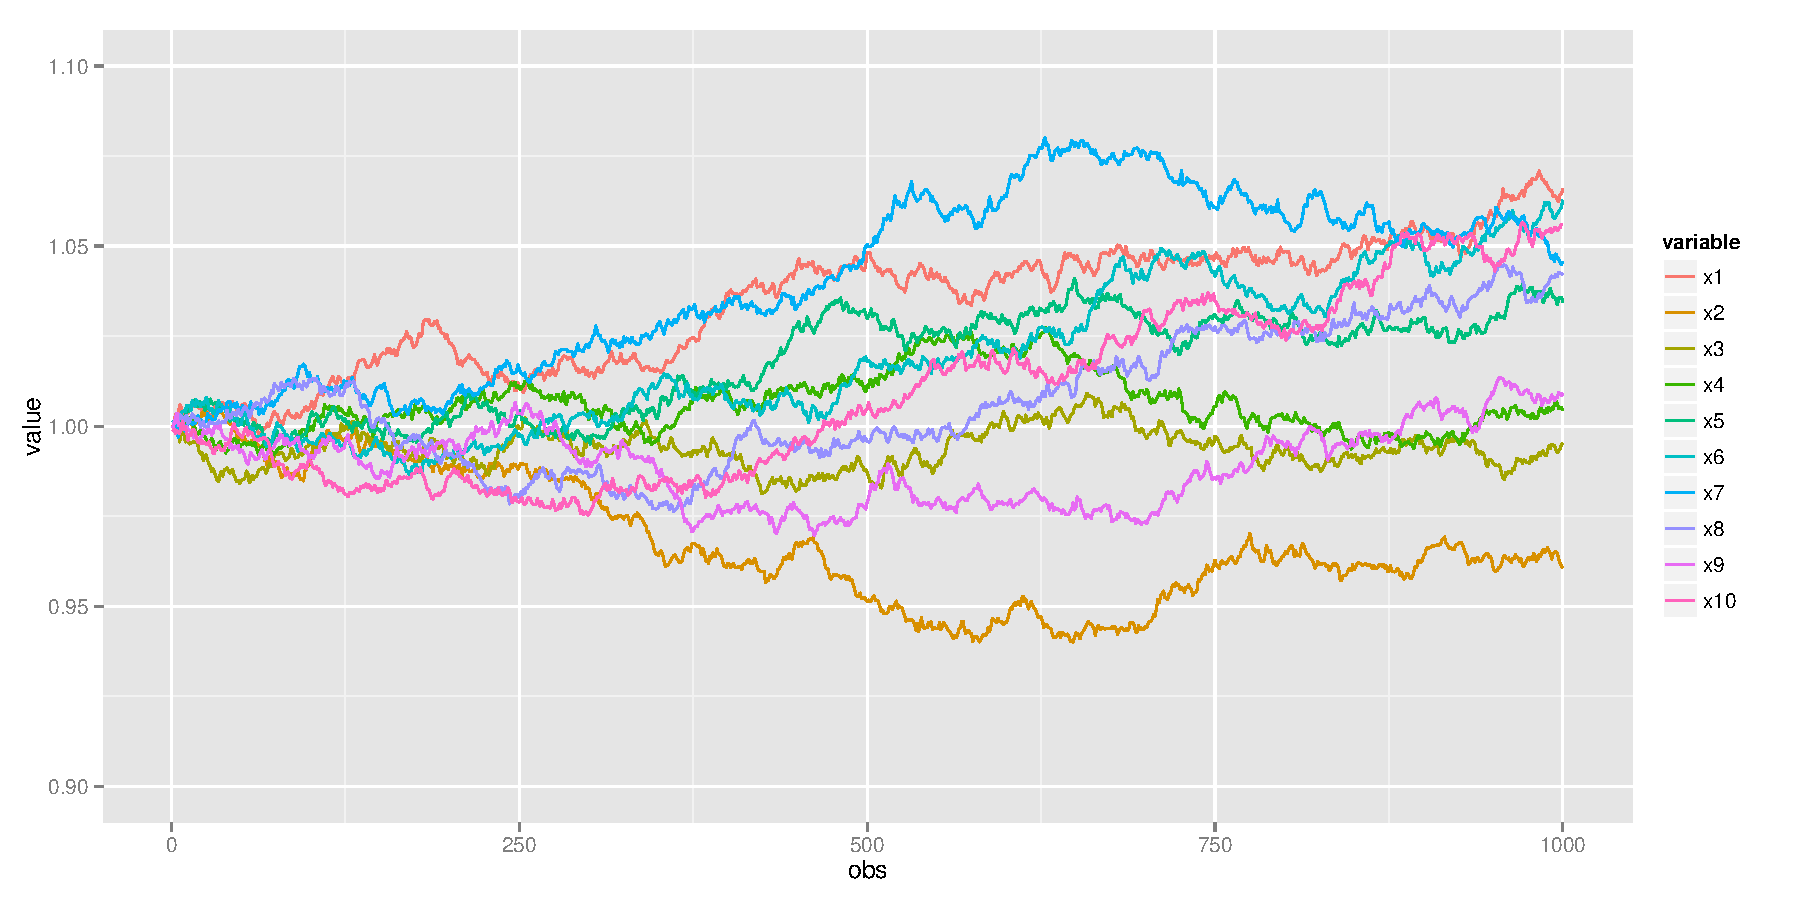
\includegraphics[width = 1.1 \textwidth]{img/rw10}
\end{center}
\end{frame}


\begin{frame}
\frametitle{Symulowany rozk�ad klasycznego estymatora zmienno�ci}
\begin{center}
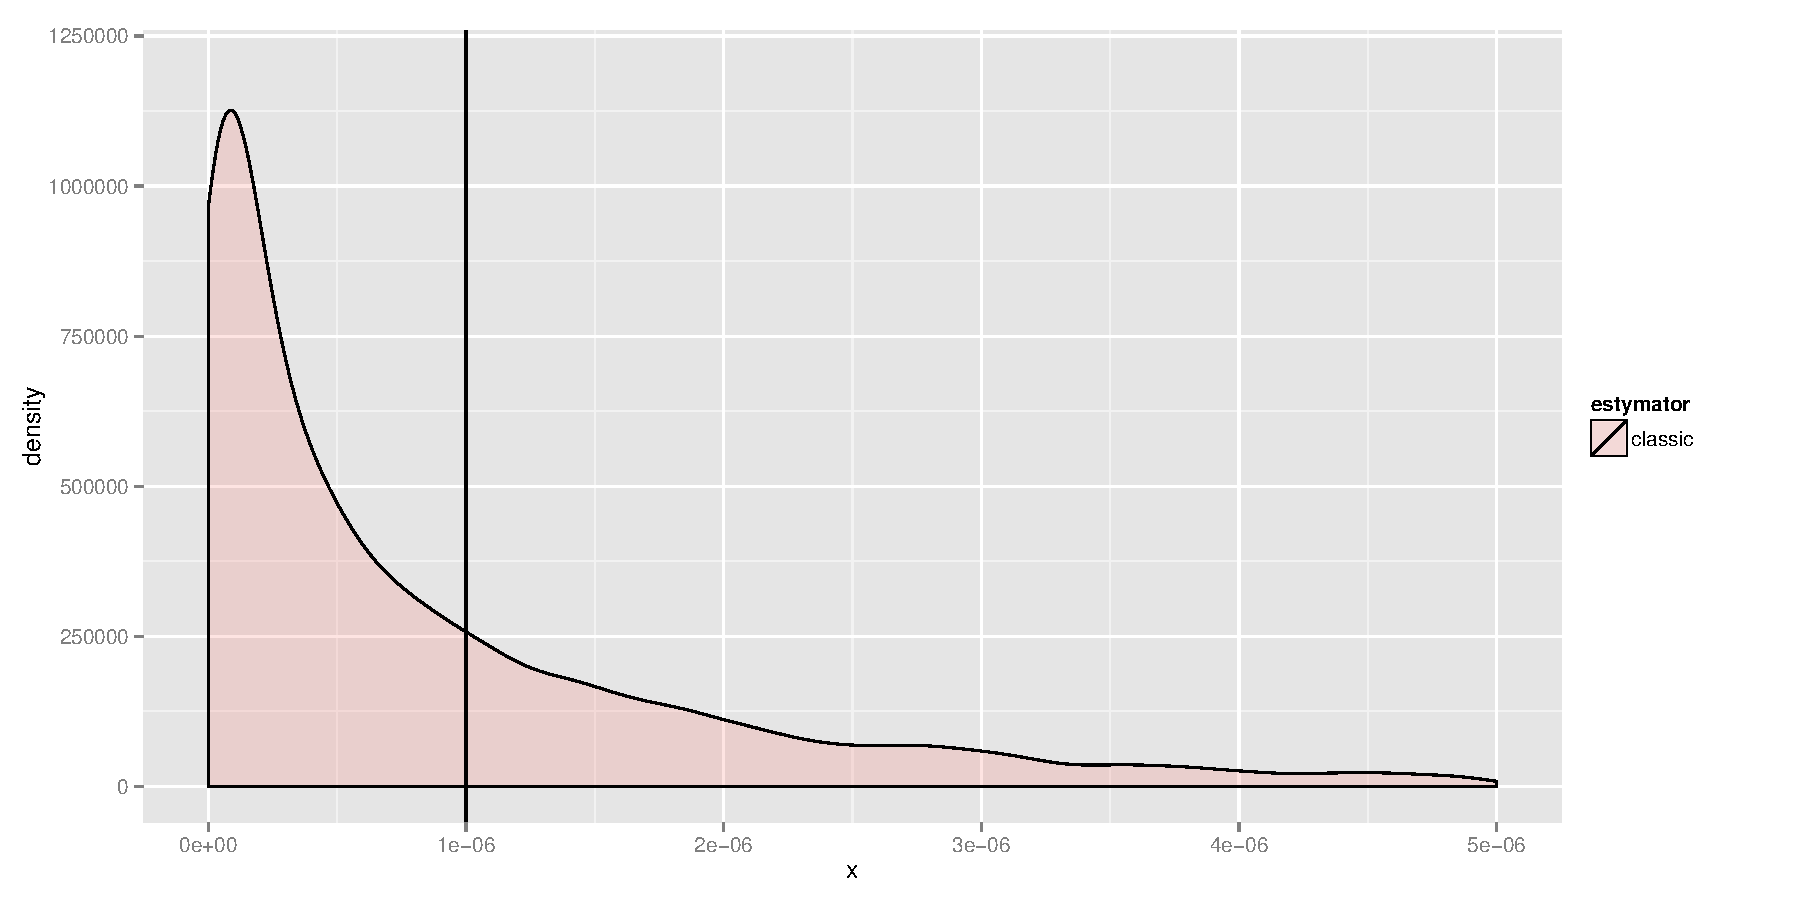
\includegraphics[width = 1.1 \textwidth]{img/plot1}
\end{center}
\end{frame}



\begin{frame}
\frametitle{Estymator $D_l$ Parkinsona (1980)}
\begin{itemize}
\item zamiast mierzy� $x(n)$ dla $n = 0, 1, 2, 3, \dots$ obserwujemy r�nic� $l$ mi�dzy logarytmami maksymalnej i minimalnej ceny wewn�trz danego interwa�u
$$
\hat{\sigma}^2_{P} = \frac{1}{4 \log 2}(\log H_t - \log L_t)^2
$$
gdzie $H_t$ i $L_t$ to odpowiednio ceny maksymalne i minimalne. \pause
\item intuicja: taki zakres powinien by� bardziej efektywnym pomiarem wariancji, w por�wnaniu ze zmian� ceny mi�dzy dwoma arbitralnie wybranymi miejscami w czasie (tj. pocz�tkiem i ko�cem danego interwa�u).
\end{itemize}
\end{frame}

\begin{frame}
\frametitle{Estymator $D_l$ Parkinsona (1980)}
\begin{itemize}
\item Rozk�ad i w�asno�ci zakresu zmian $l$ s� znane. Zachodzi m. in.:
$$
E[l^p] = \frac{4}{\sqrt{\pi}}\Gamma\bigg(\frac{p+1}{2}\bigg)\bigg(1-\frac{4}{2^p}\bigg)\zeta(p-1)(2Dt)^{p/2}
$$
gdzie $p\geq $, a $\zeta(x)$ jest funkcj� zeta Riemanna.
\item za� w szczeg�lno�ci mamy:
$$
E[l] = \sqrt{8Dt/\pi}
$$
oraz
$$
E[l^2] = (4\log 2)Dt
$$
\end{itemize}
\end{frame}


\begin{frame}
\frametitle{Estymator $D_l$ Parkinsona (1980)}
\begin{itemize}
\item dla interwa�u jednostkowego zachodzi tak�e:
$$
D = 0.393 (E[l])^2 = 0.361 E[l^2]
$$
\item mamy zatem relacj�:
$$
E[l^2] = 1.09 (E[l])^2
$$
kt�ra jest wygodna przy testowaniu tego, czy obserwowane zakresy zmian $l$ pochodz� z procesu b��dzenia losowego
\item w rezultacie, maj�c zbi�r zakres�w zmian $(l_1, l_2, \cdots, l_n)$ obserwowanych w $n$ jednostkowych interwa�ach, estymatorem wariancji $D$ jest:
$$
D_l = \frac{0.361}{n}\sum_{i=1}^nl_i^2
$$
\end{itemize}
\end{frame}


\begin{frame}
\frametitle{por�wnanie estymator�w $D_x$ i $D_l$}
\begin{itemize}
\item wariancja estymatora $D_x$
$$
E[(D_x - D)^2] = \bigg[\frac{E(x^4)}{E(x^2)}-1\bigg]\frac{D^2}{N_x}=\frac{2D^2}{N_x}
$$
\item wariancja estymatora $D_l$
$$
E[(D_l - D)^2] = \bigg[\frac{E(l^4)}{E(l^2)}-1\bigg]\frac{D^2}{N_l}=\frac{0.41D^2}{N_l}
$$
\item A zatem, wariancje estymator�w zbli�one je�li zachodzi:
$$
N_x\approx 5N_l
$$
co oznacza, �e stosuj�c $D_l$ zamiast $D_x$ mo�emy zredukowa� liczb� obserwacji o ok. \hl{80\%} zachowuj�c t� sam� precyzj� estymatora!
\end{itemize}
\end{frame}




\begin{frame}
\frametitle{Symulowany rozk�ad estymatora Parkinsona (1980)}
\begin{center}
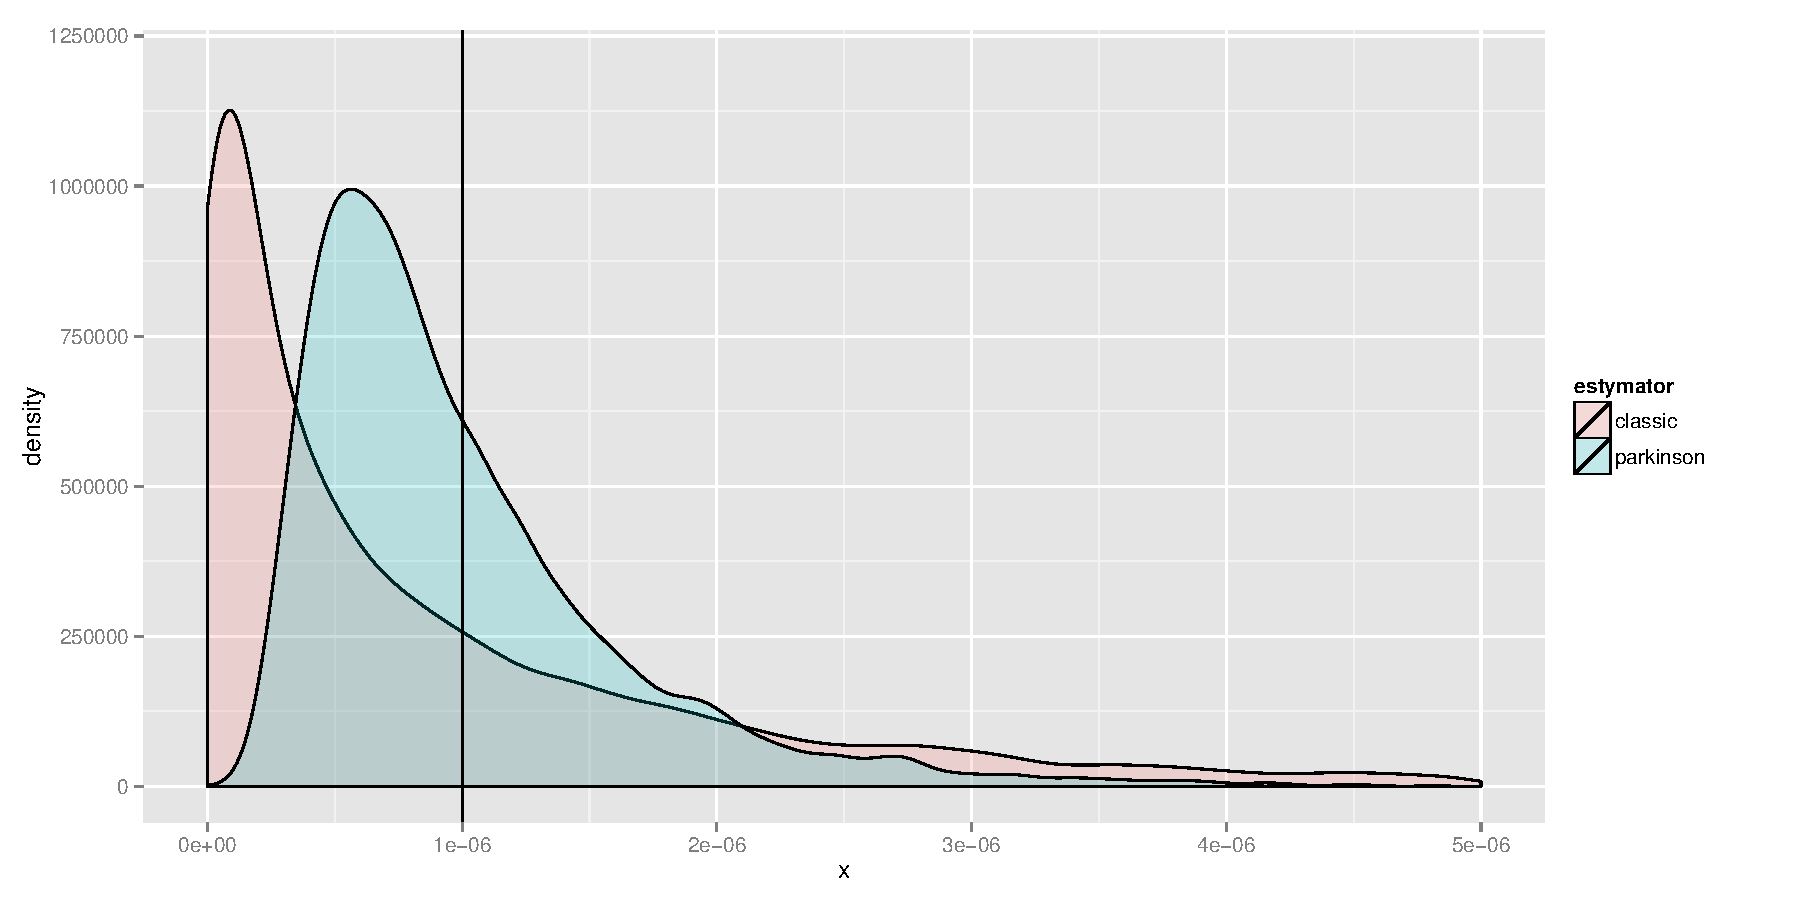
\includegraphics[width = 1.1 \textwidth]{img/plot2}
\end{center}
\end{frame}



\begin{frame}
\frametitle{Inne estymatory oparte na zakresie zmian}
\begin{itemize}
\item Estymator Osbanda (2007)
\begin{eqnarray}
\hat{\sigma}^2_{\mathrm{Osb}} &=& 0.84 (\log H_t - \log L_t) - \nonumber \\
&& - 0.39 |\log C_t - \log O_t| \nonumber
\end{eqnarray}
gdzie $O_t$ i $C_t$ to odpowiednio ceny otwarcia i zamkni�cia w interwale $t$.\pause
\item Estymator Garmana-Klassa (1980)
\begin{eqnarray}
\hat{\sigma}^2_{\mathrm{GK}} &=& 0.5[\log H_t - \log L_t]^2 - \nonumber \\
&& - (2\log 2 - 1)[\log C_t - \log O_t]^2 \nonumber \pause
\end{eqnarray}
\item Estymator Rogersa \& Satchella (1991)
\begin{eqnarray}
\hat{\sigma}^2_{\mathrm{RS}} &=& 
\log(H_t/O_t)[\log(H_t/O_t) - \log(C_t/O_t)] + \nonumber \\ 
&& +
\log(L_t/O_t)[\log(L_t/O_t) - \log(C_t/O_t)] \nonumber
\end{eqnarray}
\end{itemize}

\end{frame}



\begin{frame}
\frametitle{Symulowany rozk�ad estymatora Osbanda (2007)}
\begin{center}
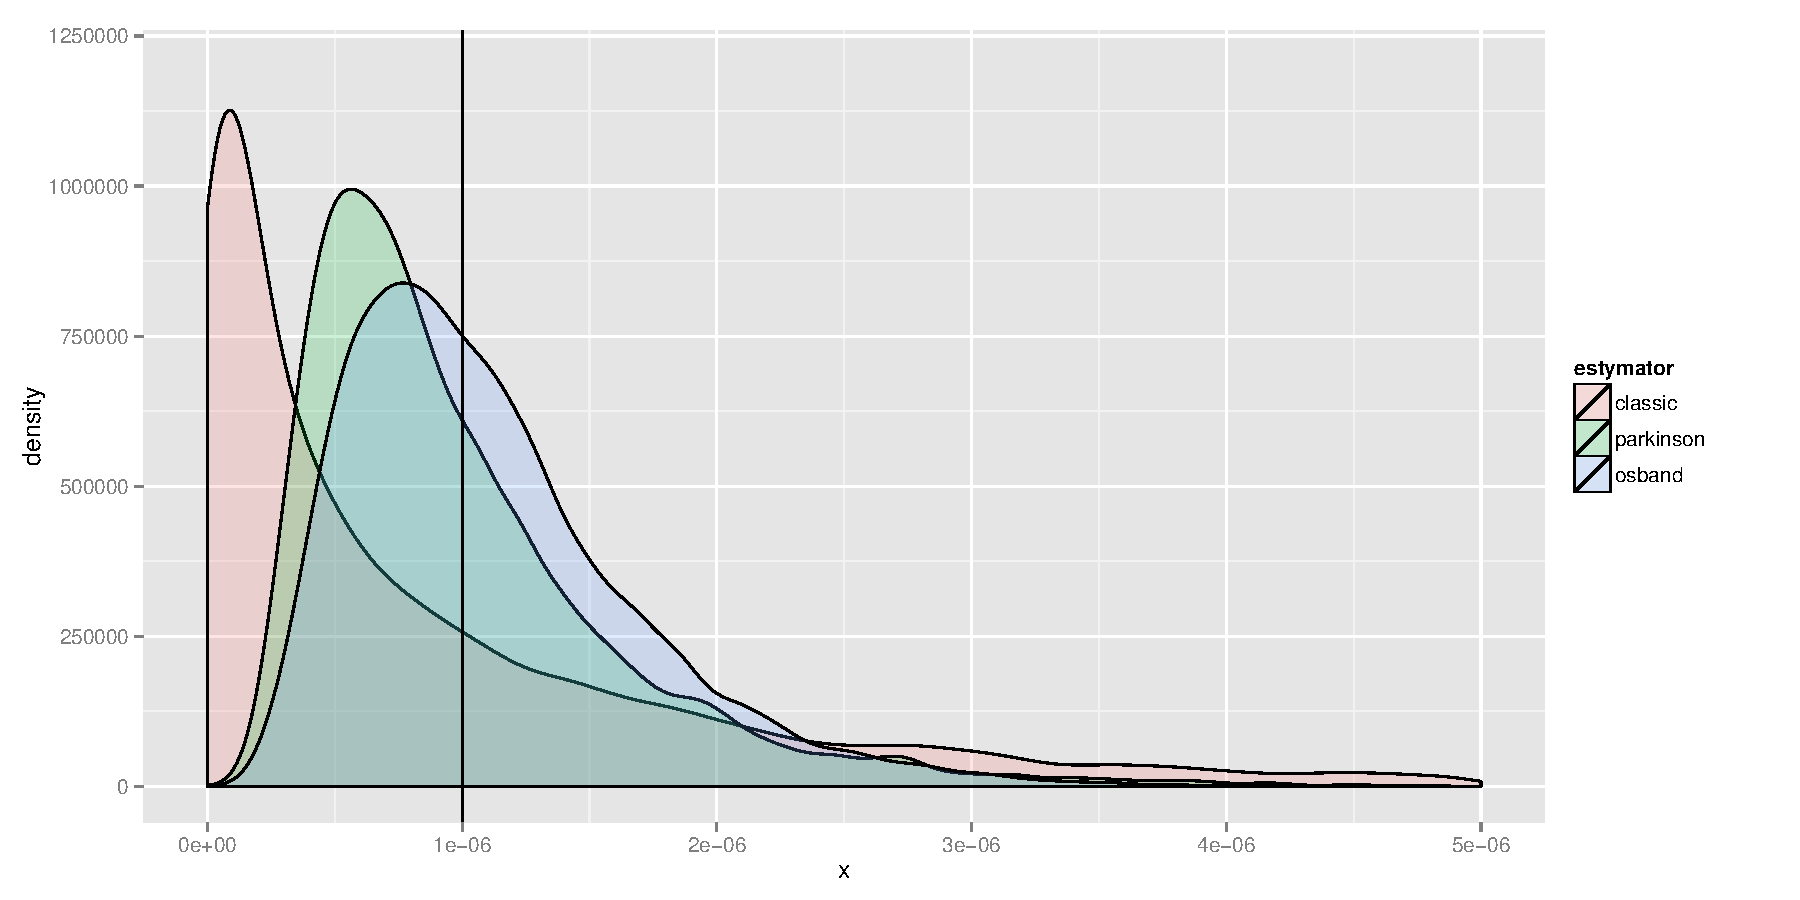
\includegraphics[width = 1.1 \textwidth]{img/plot3}
\end{center}
\end{frame}


\begin{frame}
\frametitle{Symulowany rozk�ad estymatora Garmana-Klassa (1980)}
\begin{center}
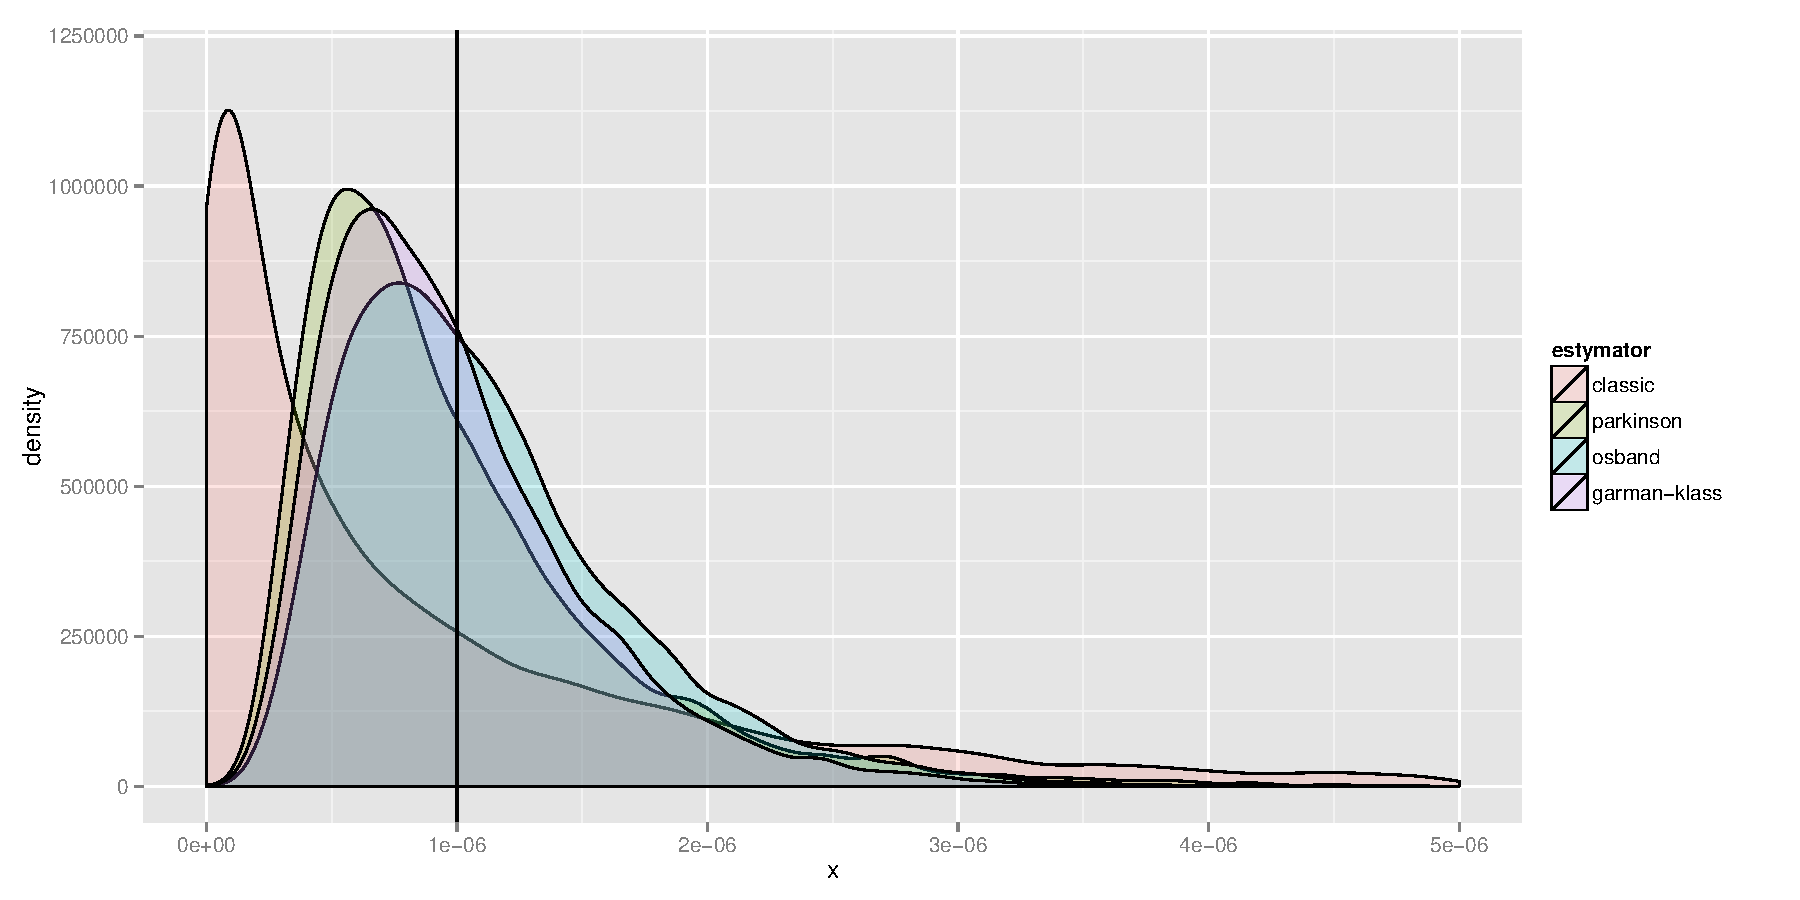
\includegraphics[width = 1.1 \textwidth]{img/plot4}
\end{center}
\end{frame}


\begin{frame}
\frametitle{Symulowany rozk�ad estymatora Rogersa-Satchella (1991)}
\begin{center}
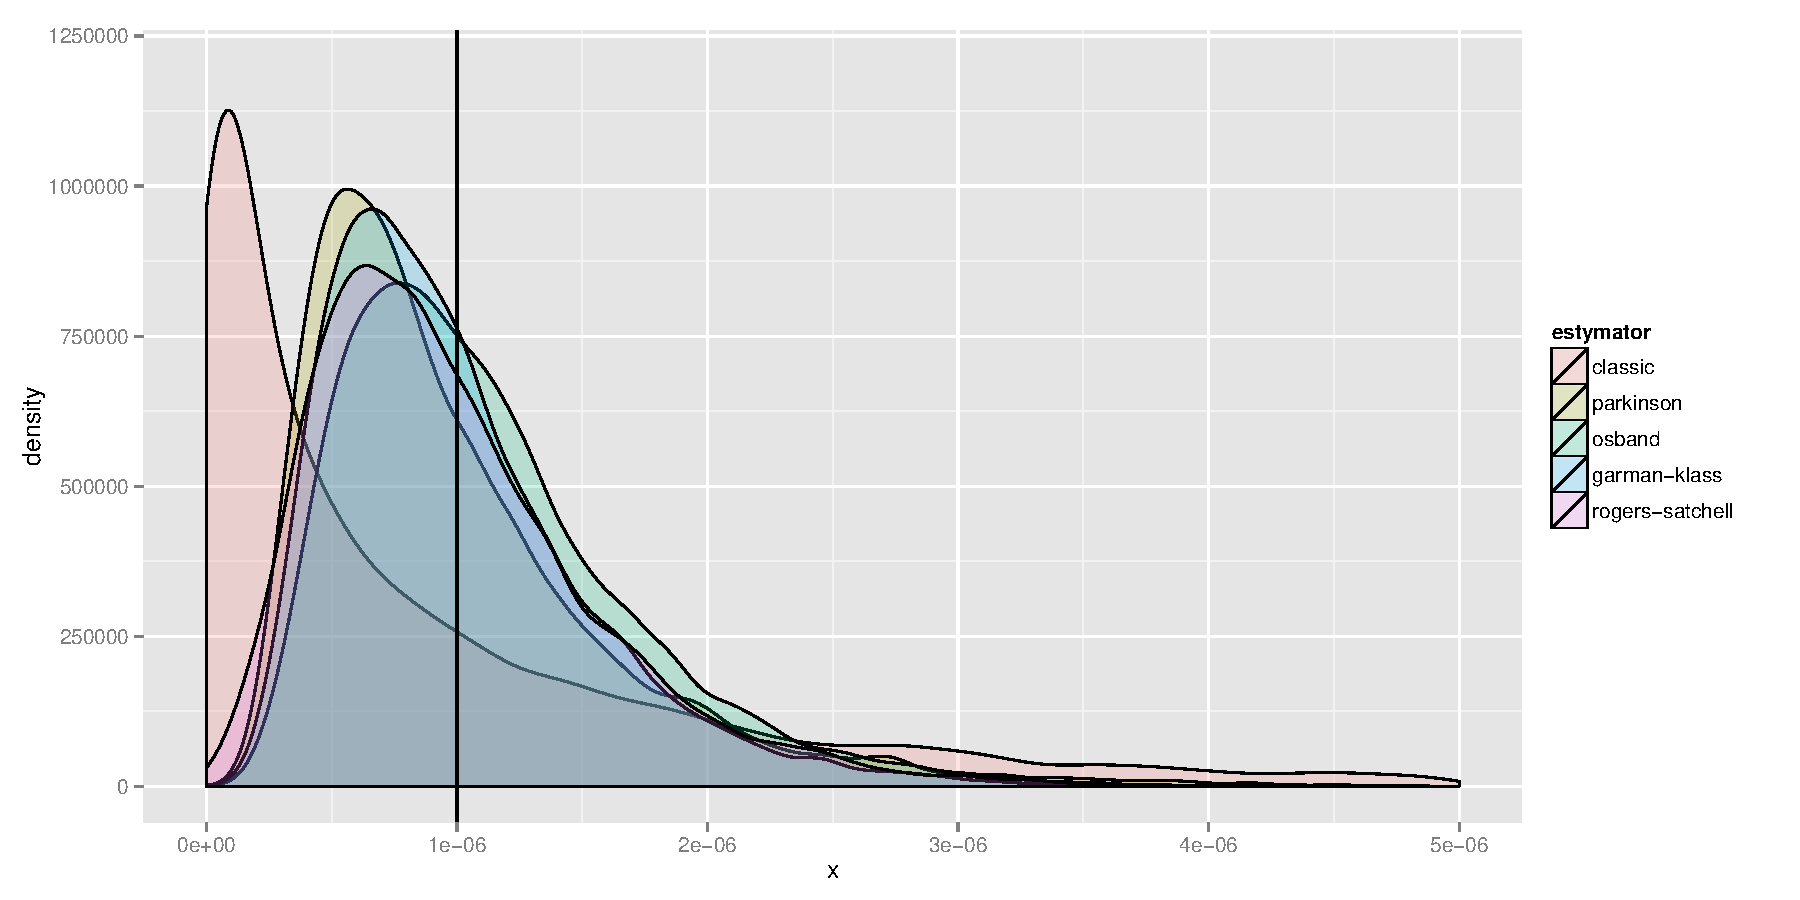
\includegraphics[width = 1.1 \textwidth]{img/plot5}
\end{center}
\end{frame}



\begin{frame}
\frametitle{Statystyki pr�bkowe estymator�w zmienno�ci}
prawdziwa warto�� $\sigma^2 = 1.0\times 10^{-6}$\\
\quad \\

\begin{tabular}{|l|c|c|c|c|c|}
\hline
 & �rednia        & odch. std. & odch. std.     & redukcja\\ 
 & $\times 10^{6}$ & $\times 10^{6}$  & do klasycznego & obs.    \\ 
\hline  
klasyczny           & 1.02 & 1.44  & - & -         \\ 
Parkinson           & 0.99 & 0.65 & 45\%  & 79.8\%    \\ 
Osband              & 1.11 & 0.57 & 40\%  & 84.2\%    \\ 
Garman-Klass        & 0.99 & 0.52 & 37\%  & 87.9\%    \\ 
Rogers-Satchell     & 0.99 & 0.57 & 40\%  & 84.2\%    \\ 
\hline
\end{tabular} 
\end{frame}


\begin{frame}
\frametitle{Uwagi do referatu Tomka Skoczylasa}
\begin{itemize}
\item Czy model RHARCH mo�e by� szacowany za pomoc� powszechnie dost�pnych pakiet�w statystycznych? 
\item Czy MSE prognoz r�ni� si� istotnie od siebie? \\
Warto rozwa�y� raportowanie odch. std. miar MSE.
\item Jak zdefiniowana jest miara QLIKE?
\item B��dy w oznaczeniach w r�wnaniach?\\
Model RGARCH(1,1)
\begin{columns} 
\begin{column}[c]{4cm} 
\begin{eqnarray}
r_t &=& \mu + \varepsilon_t \nonumber \\
\varepsilon_t &\sim& N\Big(0,\frac{1}{4\log2}\lambda_t^2\Big) \nonumber \\
\lambda_t &=& \omega + \alpha R_{t-1} + \beta\lambda_{t-1} \nonumber \\
R_{t-1} &=& \log(H_{t-1}/L_{t-1}) \overset{?}{=} \lambda_{t-1} \nonumber
\end{eqnarray}
\end{column} 
\begin{column}[c]{4cm} 
$$
\sigma_{\mathrm{P}}^2 = \frac{1}{4 \log 2}\Big(\log(H_t/L_t)\Big)^2
$$
\end{column} 
\end{columns} 
\end{itemize}
\end{frame}






%%%%%%%%%%%%%%%%%%%%%%%%%%%%%%%%%%%%%%%%%%%%%%%%%%%%%%%%%%%%%%%%%%%%%%%%%%%%%%%%%%%%%%%%%%%%
\begin{frame}
	\frametitle{}
	\begin{block}{\begin{center}\huge Dzi�kuj�!\end{center}}
\begin{center}
\vspace{2mm}
Pawe� Sakowski\\
\texttt{sakowski@wne.uw.edu.pl}\\
\end{center}
	\end{block}
\end{frame}

\end{document}

